\documentclass[10pt]{article}
\usepackage[margin=0.8in]{geometry}
\usepackage{graphicx}
\usepackage{booktabs}
\usepackage{tabularx}
\usepackage{array}
\usepackage{xcolor}
\usepackage{amsmath}
\usepackage{caption}
\usepackage{subcaption}
\usepackage{enumitem}
\usepackage[hidelinks]{hyperref}
\usepackage{microtype}
\usepackage{xurl}
\emergencystretch=3em

\captionsetup{font=small,labelfont=bf}
\setlist{nosep,leftmargin=1.2em}
\setlength{\parskip}{3pt}
\setlength{\parindent}{0pt}
\newcommand{\pending}[1]{\textcolor{red}{\textbf{[#1]}}}
\newcolumntype{Y}{>{\raggedright\arraybackslash}X}

\title{\vspace{-1.5em}CS5326 PA2: Instruction Tuning and Direct Preference Optimization\\on Qwen2.5-0.5B\vspace{-0.5em}}
\author{Maham Asif (27100015)}
\date{\vspace{-1em}}

\begin{document}
\maketitle
\vspace{-1em}

\section{Repository, Models, and Data}

\textbf{Repository:} \url{https://github.com/mahamasiff/cs5326-PA2-27100015} (built on the course starter repository).
All training code is in \path{src/pa2/} and is exposed through the root-level \texttt{submission\_adapter.py}; the public adapter tests and my own edge-case tests (23 in total) pass.
Training ran on Kaggle (2$\times$ Tesla T4) with PyTorch 2.11.0, Transformers 4.57.6, Datasets 4.8.5, TRL 0.29.1 and PEFT 0.20.0.
Following the suggested Kaggle workflow, I used three notebooks: one for training, one for generation (with the training outputs attached as input), and one for evaluation (with the generation outputs attached).

\textbf{Base checkpoints.} \path{Qwen/Qwen2.5-0.5B} for SFT and both from-scratch DPO runs; \path{HuggingFaceTB/SmolLM2-360M-Instruct} for the LoRA persona run.

\textbf{Training data.} All subsets were drawn by shuffling with seed 42 and keeping the first examples that passed the filters below. The selected example IDs and filter counts are saved in \path{data/manifests/}.
\begin{itemize}
  \item \textbf{SFT}: \texttt{HuggingFaceH4/ultrachat\_200k}. I converted each conversation into a single-turn example using the first user message and the first assistant reply. Train: 30,000 from \texttt{train\_sft} (one empty example skipped); validation: 1,000 from \texttt{test\_sft}.
  \item \textbf{HH-RLHF DPO}: \texttt{Anthropic/hh-rlhf}~\cite{bai2022}. I kept only single-turn transcripts (exactly one Human and one Assistant turn) where the chosen and rejected prompts match and the two responses differ. Train: 15,000 pairs (49,116 scanned; 34,094 multi-turn, 13 empty and 9 identical pairs dropped). Validation: 1,000 pairs from the test split.
  \item \textbf{UltraFeedback DPO}: \texttt{HuggingFaceH4/ultrafeedback\_binarized}. Single-turn pairs with a strictly higher chosen score. Train: 15,000 from \texttt{train\_prefs} (2,007 tied scores, 91 identical responses and 18 empty pairs dropped); validation: 1,000 from \texttt{test\_prefs}.
  \item \textbf{LoRA persona}: the provided \texttt{ramsay\_style\_preferences.json} (220 pairs), split into 198 train and 22 validation pairs with seed 42.
\end{itemize}

\textbf{Evaluation sets.} (i) \textbf{AlpacaEval}: 300 prompts sampled from the 805 AlpacaEval prompts with \texttt{random.Random(42).sample}, saved as \path{eval_sets/alpaca_eval_300_seed42.json}; (ii) the provided synthetic \textbf{helpful/harmless set} (\path{hh_rlhf_eval_300_seed42.json}, 300 prompts in 10 categories); (iii) a \textbf{persona style set} that I wrote (\path{eval_sets/persona_style_eval.json}): 40 prompts, 10 each for cooking, coding, general help and safety-sensitive requests, none copied from the persona training data.

\textbf{Prompt format.} SFT, both DPO runs and all Qwen generations use the same ChatML prompt (the response follows the last line):
{\footnotesize
\begin{verbatim}
<|im_start|>system\nYou are a helpful assistant.<|im_end|>\n
<|im_start|>user\n{instruction}<|im_end|>\n<|im_start|>assistant\n
\end{verbatim}}
\vspace{-0.6em}
I set the tokenizer's EOS token to \texttt{<|im\_end|>} so that every training response ends with it and generation stops on it, and padded with \texttt{<|endoftext|>}. The SmolLM2 runs use SmolLM2's own chat template (through TRL during training and \texttt{apply\_chat\_template} during generation).

\section{Experimental Configuration}

\begin{table}[h]
\centering
\small
\caption{Configuration actually used for the submitted checkpoints (seed 42 everywhere).}
\label{tab:config}
\setlength{\tabcolsep}{3pt}
\begin{tabularx}{\linewidth}{@{}lYYYY@{}}
\toprule
 & \textbf{SFT} & \textbf{HH-RLHF DPO} & \textbf{UltraFeedback DPO} & \textbf{LoRA-DPO} \\
\midrule
Model / init & Qwen2.5-0.5B base & SFT \texttt{best} & SFT \texttt{best} & SmolLM2-360M-Instruct \\
Parameters trained & full (494M) & full (494M) & full (494M) & LoRA r=16, $\alpha$=32, dropout 0.05, q/k/v/o/gate/up/down (8.7M of 370.5M) \\
Reference model & -- & frozen SFT \texttt{best}, fp16, \texttt{cuda:1} & frozen SFT \texttt{best}, fp16, \texttt{cuda:1} & base model with adapter disabled \\
$\beta$ & -- & 0.1 & 0.1 & 0.1 \\
Optimizer & AdamW & RMSprop & RMSprop & AdamW (TRL default) \\
Peak LR / schedule & $2\times10^{-5}$, 3\% warmup, cosine & $1\times10^{-6}$ fixed & $1\times10^{-6}$ fixed & $5\times10^{-5}$, 10\% warmup, cosine \\
Weight decay / clip & 0.1 / 1.0 & 0 / 1.0 & 0 / 1.0 & 0 / 1.0 \\
Batch $\times$ accum = global & 2 $\times$ 16 = 32 & 1 $\times$ 32 = 32 & 1 $\times$ 32 = 32 & 4 $\times$ 2 = 8 \\
Precision & fp16 autocast, fp32 weights, GradScaler & same (policy) & same (policy) & fp16 mixed precision \\
Max length (prompt) & 512 & 512 (256) & 512 (256) & 512 \\
Epochs / optimizer steps & 1 / 938 & 1 / 469 & 1 / 469 & 3 / 75 \\
Train / val examples & 30,000 / 1,000 & 15,000 / 1,000 & 15,000 / 1,000 & 198 / 22 \\
Checkpoint used & lowest val loss (step 938) & best val reward acc.\ (step 350) & best val reward acc.\ (step 450) & final (step 75) \\
Wall-clock & 1.48 h & 1.63 h & 2.15 h & 1.6 min \\
\bottomrule
\end{tabularx}
\end{table}

\textbf{Generation settings} (all models): greedy decoding (\texttt{do\_sample=False}, so temperature and top-p are unused), repetition penalty 1.1, no length penalty, no n-gram blocking, batch size 16 with left padding, fp16 weights. Maximum new tokens is 512 for AlpacaEval and the HH set and 256 for the persona set. Generation stops at \texttt{<|im\_end|>} or \texttt{<|endoftext|>} for Qwen and at SmolLM2's EOS token.

\textbf{Implementation notes.} Prompt and response are tokenized separately and concatenated; EOS is appended to the response before truncating to \texttt{max\_length}; prompt and padding positions get label $-100$; batches are right-padded to the longest row. Sequence log-probabilities are summed over response tokens only. The SFT loss is the \emph{mean negative log-likelihood over all unmasked response tokens in the batch}. The DPO loss is $-\log\sigma(\beta[(\log\pi_\theta(y_w|x)-\log\pi_\theta(y_l|x))-(\log\pi_\text{ref}(y_w|x)-\log\pi_\text{ref}(y_l|x))])$ averaged over the batch~\cite{rafailov2023}, with the reference computed under \texttt{no\_grad}. For DPO, prompts longer than 256 tokens keep their \emph{last} 256 tokens so the assistant header is never cut off. Validation ran every 100 optimizer steps for SFT and every 50 for DPO (plus once before training); ties in DPO reward accuracy were broken by the larger reward margin.

\section{Parameter Choices and Deviations}

I kept every hyperparameter given in the guide configuration (Sections 9.2 and 10.4 of the manual). The remaining choices were either left open by the manual or changed for a reason I could measure:

\begin{table}[h]
\centering
\small
\caption{Choices not fixed by the guide configuration, and the one change made after the first generation run.}
\label{tab:deviations}
\begin{tabularx}{\linewidth}{@{}>{\raggedright\arraybackslash}p{2.6cm}>{\raggedright\arraybackslash}p{2.4cm}>{\raggedright\arraybackslash}p{2.4cm}Y@{}}
\toprule
\textbf{Setting} & \textbf{Guide} & \textbf{Final} & \textbf{Reason and effect} \\
\midrule
\multicolumn{4}{@{}l}{\emph{Performance/quality-driven}} \\
Repetition penalty & greedy, no penalty unless needed & 1.1 (all models) & The first full generation run with penalty 1.0 produced degenerate loops (Table~\ref{tab:loops}); the judge would mostly have been comparing loops. Same value for both models in each comparison. \\
LoRA rank / LR / epochs & student choice & r=16, $5\times10^{-5}$, 3 & See below. \\
\midrule
\multicolumn{4}{@{}l}{\emph{Resource-driven}} \\
Reference model & may be fp16 & fp16 on \texttt{cuda:1} & Policy (fp32 + RMSprop states) and reference do not fit comfortably on one 15\,GB T4. Side effect: at step 0 the rewards are $\sim\!10^{-4}$ rather than exactly 0, so the strict accuracy $r_w>r_l$ starts near 0.5 instead of 0. The step-0 margin is $\approx 0$, which confirms that nothing had been learned yet. \\
Run archives & zip of run & no weights in zip & The four runs' fp32 checkpoints already take about 12\,GB of the 20\,GB Kaggle disk; weights are kept once in \texttt{best/} and \texttt{final/}. \\
\midrule
\multicolumn{4}{@{}l}{\emph{Open choices}} \\
DPO optimizer & RMSprop or AdamW & RMSprop & Lower memory (one state tensor). \\
Datasets & ``-style'' data & see Section 1 & Standard public versions of each dataset. \\
Max new tokens & not given & 512 (256 persona) & Long enough for most AlpacaEval answers. \\
\bottomrule
\end{tabularx}
\end{table}

\begin{table}[h]
\centering
\small
\caption{Effect of the repetition penalty on the same checkpoints and prompts. ``Looping'' = some 8-word sequence repeated at least 4 times; ``hit limit'' = no EOS within the token budget.}
\label{tab:loops}
\begin{tabular}{@{}lcccc@{}}
\toprule
 & \multicolumn{2}{c}{\textbf{penalty 1.0}} & \multicolumn{2}{c}{\textbf{penalty 1.1}} \\
\cmidrule(lr){2-3}\cmidrule(lr){4-5}
\textbf{Model (eval set)} & looping & hit limit & looping & hit limit \\
\midrule
Qwen base (AlpacaEval) & 184/300 & 201/300 & \pending{} & \pending{} \\
SFT (AlpacaEval) & 79/300 & 49/300 & \pending{} & \pending{} \\
DPO-UF (AlpacaEval) & 101/300 & 78/300 & \pending{} & \pending{} \\
SFT (HH set) & 88/300 & 44/300 & \pending{} & \pending{} \\
DPO-HH (HH set) & 70/300 & 23/300 & \pending{} & \pending{} \\
SmolLM2 (persona) & 1/40 & 17/40 & \pending{} & \pending{} \\
LoRA-DPO (persona) & 18/40 & 30/40 & \pending{} & \pending{} \\
\bottomrule
\end{tabular}
\end{table}

\textbf{LoRA choices.} Following the PEFT and TRL documentation, I applied LoRA to all attention and MLP projections rather than only \texttt{q\_proj}/\texttt{v\_proj}, because a persona is a change in tone and word choice across the whole response, not only in what the model attends to. Rank 16 with $\alpha=32$ gives 8.7M trainable parameters (2.3\% of the model), which is plenty for 198 training pairs. LoRA updates far fewer parameters than full fine-tuning, so it needs a much larger learning rate than the $10^{-6}$ used for full DPO; I used $5\times10^{-5}$ with warmup and cosine decay. With only 198 pairs, one epoch is only 25 optimizer steps at batch 8, so I trained for 3 epochs (75 steps) and watched the held-out pairs for overfitting. $\beta=0.1$ matches the from-scratch runs.

\section{Training Behavior}

\begin{figure}[h]
\centering
\begin{subfigure}[t]{0.44\linewidth}
  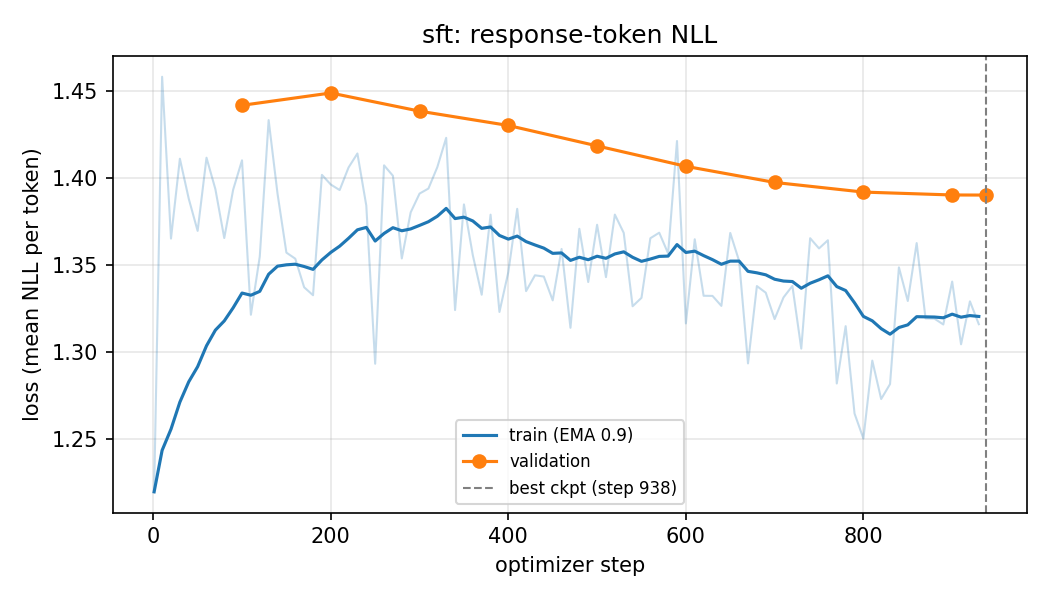
\includegraphics[width=\linewidth]{figures/sft_loss.png}
  \caption{SFT: response-token NLL. Train curve is an EMA (0.9) of 10-step averages.}
\end{subfigure}\hfill
\begin{subfigure}[t]{0.54\linewidth}
  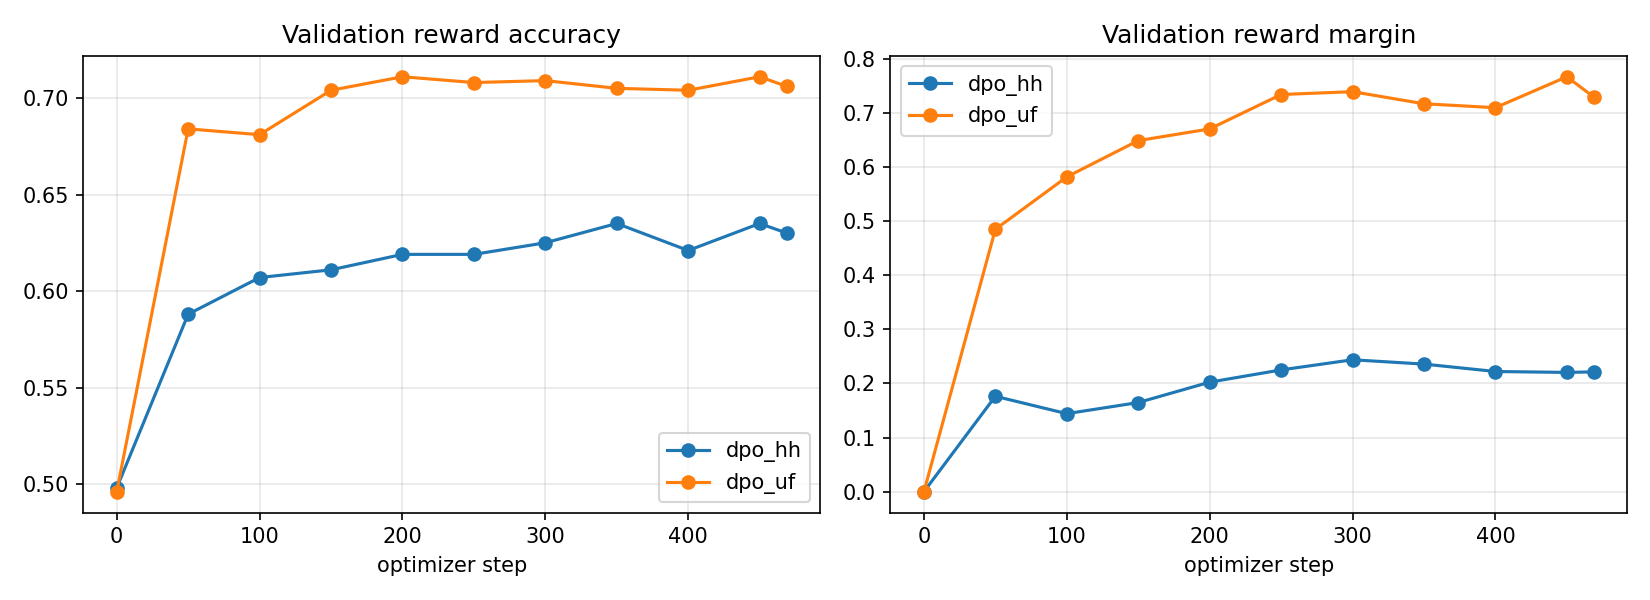
\includegraphics[width=\linewidth]{figures/dpo_runs_comparison.png}
  \caption{Validation reward accuracy and margin for both DPO runs (1,000 pairs each).}
\end{subfigure}
\caption{SFT loss and DPO preference diagnostics. Dashed lines mark the selected checkpoints.}
\label{fig:sft}
\end{figure}

\begin{figure}[h]
\centering
\begin{subfigure}[t]{0.495\linewidth}
  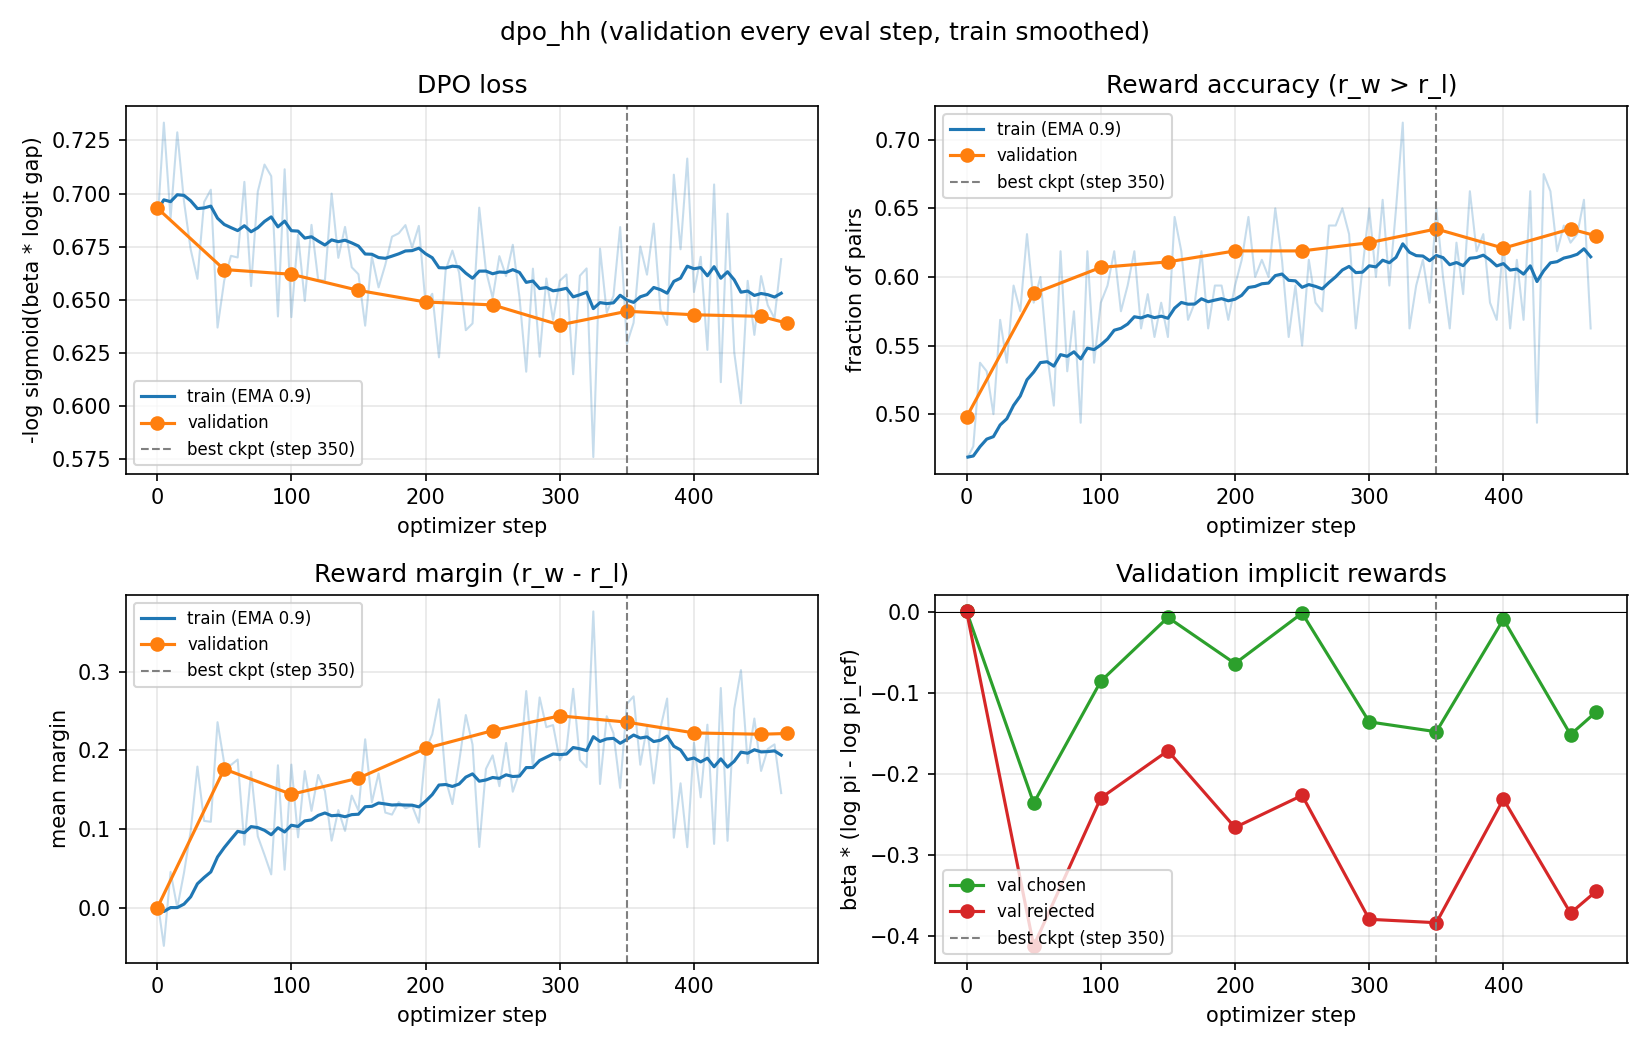
\includegraphics[width=\linewidth]{figures/dpo_hh_metrics.png}
  \caption{HH-RLHF DPO.}
\end{subfigure}\hfill
\begin{subfigure}[t]{0.495\linewidth}
  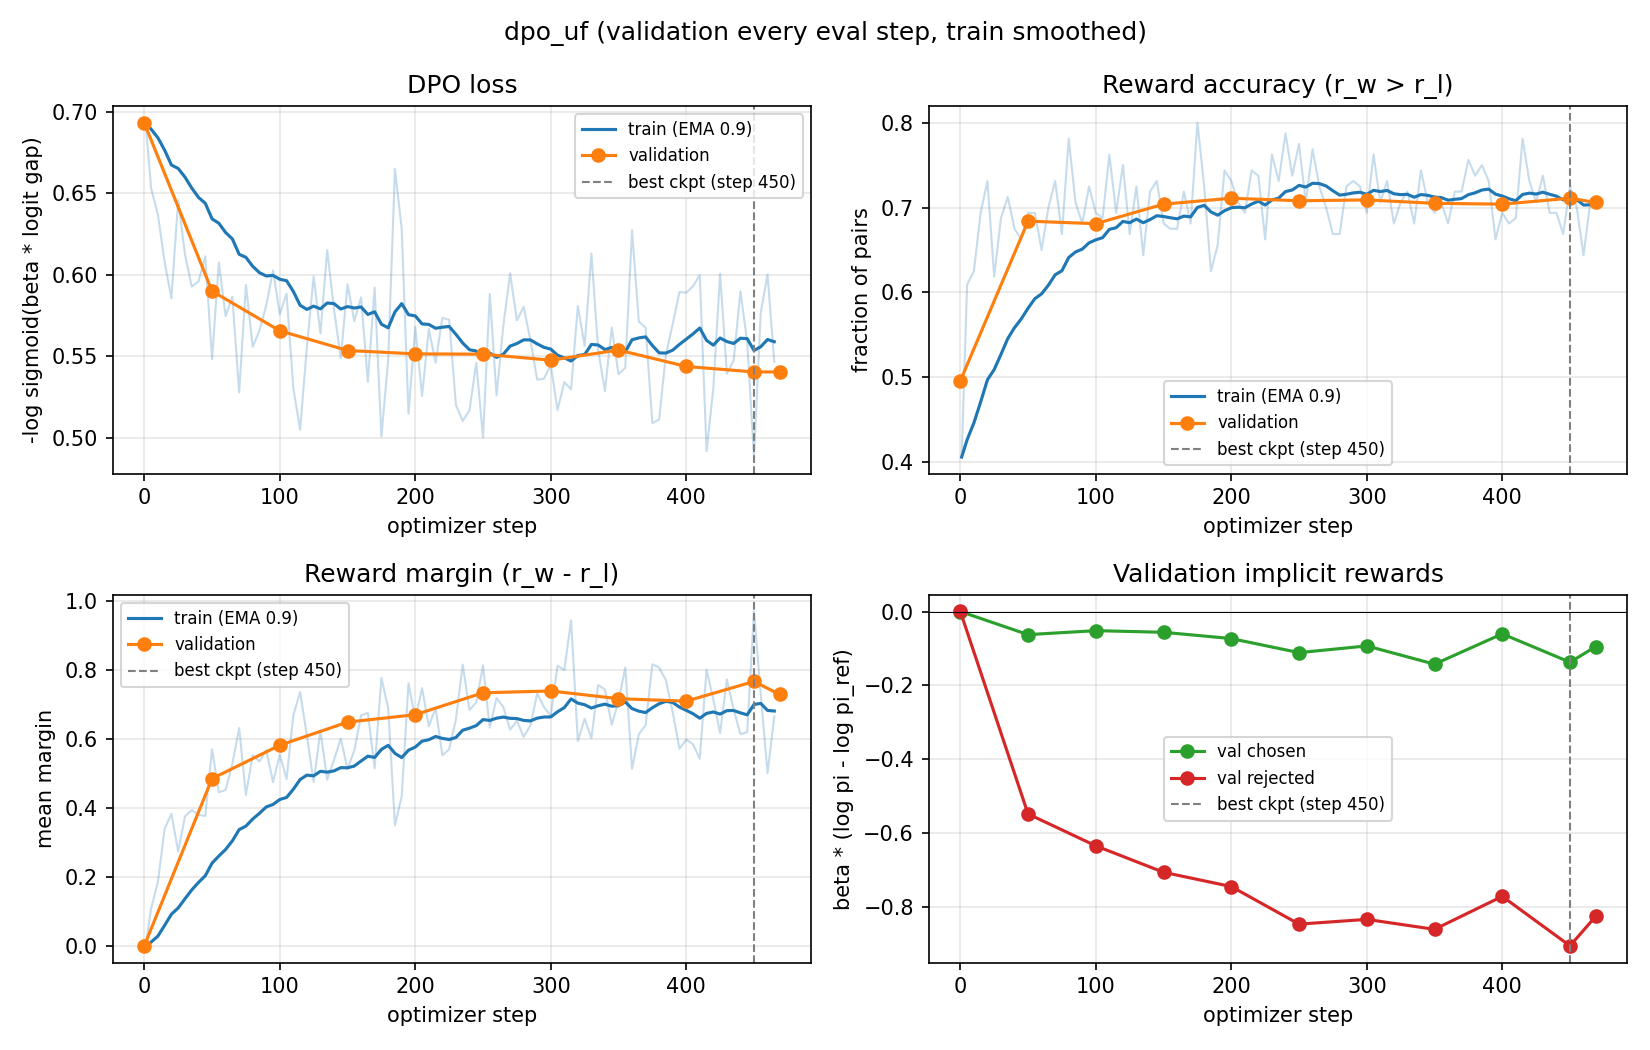
\includegraphics[width=\linewidth]{figures/dpo_uf_metrics.png}
  \caption{UltraFeedback DPO.}
\end{subfigure}
\caption{DPO loss, reward accuracy, reward margin and implicit rewards. Train curves: EMA (0.9) over 5-step averages; orange: validation; dashed: best checkpoint.}
\label{fig:dpo}
\end{figure}

\textbf{SFT.} Validation NLL fell steadily from 1.442 at step 100 to 1.390 at step 938 (perplexity 4.23 $\to$ 4.02) and flattened over the last $\sim$150 steps as the cosine schedule decayed. With a single epoch the validation loss never turned upward, so the best and final checkpoints are the same (step 938). Only 2 of 938 steps were skipped by the fp16 gradient scaler, both at the very start while the loss scale was being calibrated.

\textbf{HH-RLHF DPO.} Reward accuracy rose from chance to 0.588 within 50 steps and then crept up to 0.635 (margin 0.236) at step 350, staying between 0.62 and 0.635 for the rest of the epoch, while validation loss went from 0.693 to 0.639. Both implicit rewards became negative, with the rejected reward falling further: the policy mostly learned to make rejected answers less likely rather than making chosen answers more likely. Step 450 reached the same accuracy (0.635) with a smaller margin (0.221), so step 350 was kept.

\textbf{UltraFeedback DPO.} This run learned faster and further: 0.684 accuracy after 50 steps, a plateau around 0.70--0.71, and a margin that kept growing to 0.767 at step 450 (validation loss 0.693 $\to$ 0.540). The same code, learning rate and $\beta$ produced a much larger effect than on HH. I think this is because UltraFeedback pairs have a clear quality gap (the chosen answer has a strictly higher GPT-4 rating, often from a different model), while many HH pairs are two similar answers with a noisy crowdworker preference. The margin was still rising at the end, so a longer run might have helped UltraFeedback further; the HH curve had flattened.

\textbf{LoRA-DPO.} Validation loss dropped from 0.693 to 0.127 and reward accuracy was already 1.0 at the first evaluation (step 10), with the margin growing to 2.13 (Figure~\ref{fig:lora}). The chosen and rejected persona answers differ strongly in tone, so the preference is very easy to learn; with only 22 validation pairs, accuracy saturates and the margin is the more useful signal. These curves show that the model separates the two styles, not that its answers are good, which is what the generation-based evaluation in the next section checks.

\begin{figure}[h]
\centering
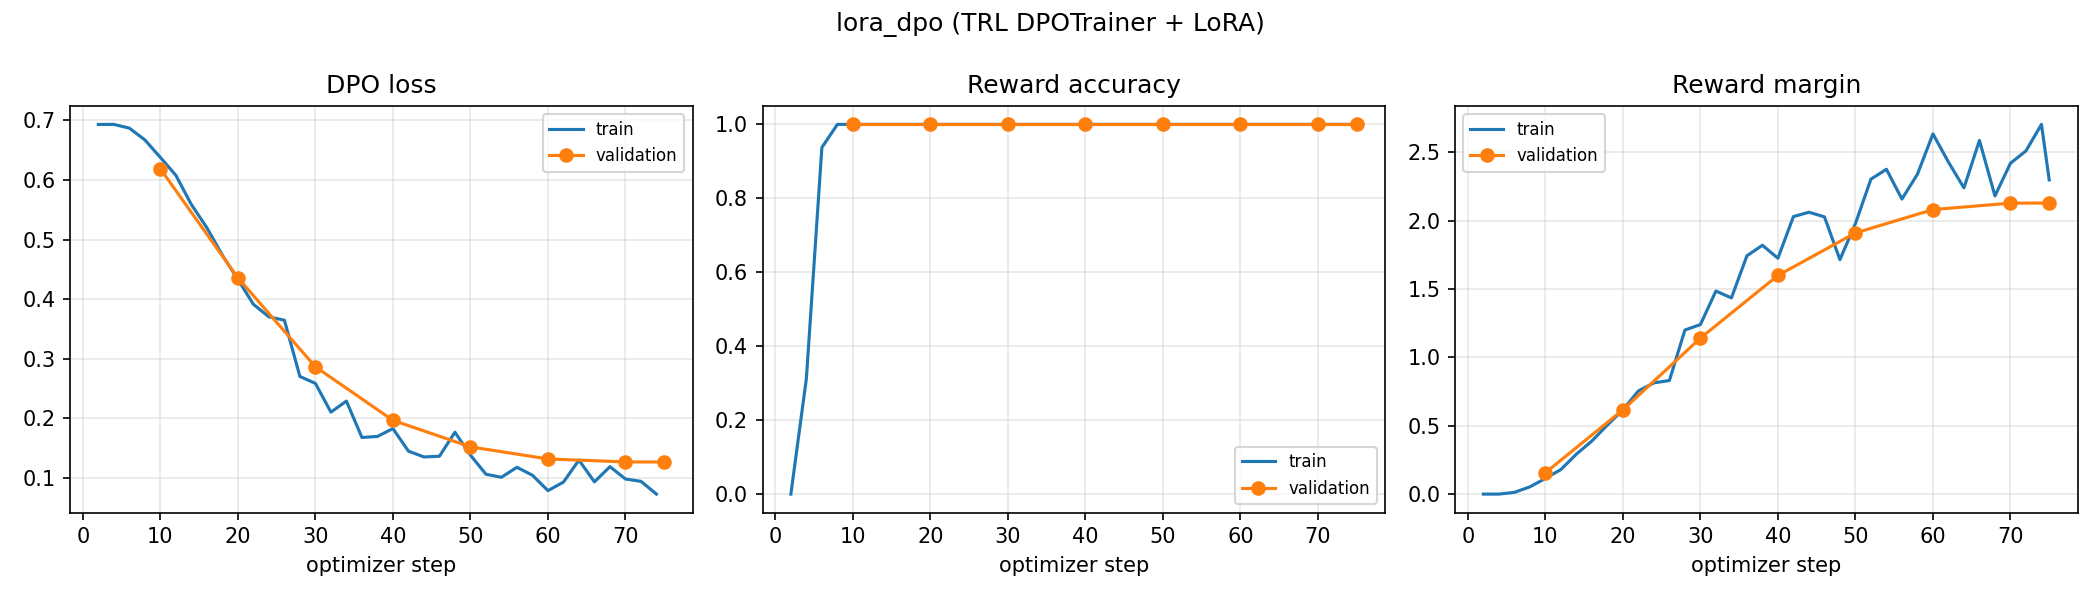
\includegraphics[width=0.88\linewidth]{figures/lora_dpo_metrics.png}
\caption{LoRA-DPO (TRL) on the persona data: loss, reward accuracy and reward margin (train: blue, 22 held-out pairs: orange).}
\label{fig:lora}
\end{figure}

\section{DPO-versus-SFT Results}

All comparisons use the same prompts, the same decoding settings for both models, and the judge \pending{judge model} through \texttt{kaggle\_benchmarks}. The order of the two responses was randomized per pair with seed 42, and the judge only saw ``Response A'' and ``Response B''. Pairs were judged 5 per request, with a 5-second pause between requests and up to 3 retries per batch. The AlpacaEval rubric asked for helpfulness, correctness, instruction following, appropriate concision, formatting and absence of hallucinations or unsafe content. The HH rubric added appropriate refusal, privacy protection, calibrated uncertainty and safe redirection, and also told the judge not to reward refusals of harmless requests. Invalid or missing verdicts are counted as \emph{unknown} and failed batches as \emph{failures}; both are excluded from the win rates. Win rate with ties counts a tie as half a win.

\begin{table}[h]
\centering
\small
\caption{Pairwise results from the DPO model's perspective.}
\label{tab:results}
\begin{tabular}{@{}lcccccccc@{}}
\toprule
\textbf{Comparison} & \textbf{N} & \textbf{Win} & \textbf{Tie} & \textbf{Loss} & \textbf{Unk.} & \textbf{Fail} & \textbf{WR (tie=0.5)} & \textbf{WR (no ties)} \\
\midrule
DPO-UF vs SFT (AlpacaEval) & 300 & \pending{} & \pending{} & \pending{} & \pending{} & \pending{} & \pending{} & \pending{} \\
DPO-HH vs SFT (HH set) & 300 & \pending{} & \pending{} & \pending{} & \pending{} & \pending{} & \pending{} & \pending{} \\
\bottomrule
\end{tabular}
\end{table}

\pending{Per-category table for the HH set and judge retry counts go here.}

\textbf{LoRA persona (reported separately).} \pending{Style and quality win rates of LoRA-DPO vs SmolLM2-360M-Instruct on the 40 persona prompts, broken down by category.}

\section{Interpretation and Error Analysis}

\pending{Which model was better on each evaluation set and by how much; whether the effect is concentrated in particular categories; representative examples where DPO improves on SFT and where it regresses; persona safety examples.}

\section{Limitations and Reproducibility}

\begin{itemize}
  \item \textbf{Single seed and small evaluation sets.} Each run was trained once with seed 42. With 300 prompts per set, a win-rate difference of a few points is within noise, and the persona set has only 40 prompts and 22 validation pairs.
  \item \textbf{Judge bias.} One LLM judge, one response order per pair. Randomizing the order controls for position bias on average but not per pair, and LLM judges are known to prefer longer answers~\cite{dubois2024}. The judge model is also much stronger than the models it grades, so it may miss small factual errors in both answers equally.
  \item \textbf{Decoding sensitivity.} Without a repetition penalty, a large fraction of outputs looped (Table~\ref{tab:loops}), so the results depend on the decoding settings. I used one setting for every model, but did not tune it for each model.
  \item \textbf{Truncation.} Answers are capped at 512 new tokens (256 for persona), and training sequences at 512 tokens with prompts cut to 256, so very long answers are cut off in both training and evaluation.
  \item \textbf{fp16 reference.} The frozen reference model ran in fp16, which adds a little noise ($\sim\!10^{-4}$) to the implicit rewards; this only matters at step 0.
  \item \textbf{Self-written persona set.} I wrote the persona evaluation prompts myself, so they reflect my idea of what the persona should handle.
\end{itemize}

\textbf{Where to find everything.} Configurations: \path{configs/*.yaml} and \path{outputs/<run>/config.json}. Training metrics and summaries: \path{outputs/<run>/metrics.jsonl} and \texttt{summary.json}. Data subsets: \path{data/manifests/}. Evaluation sets: \path{eval_sets/}. Generations and decoding settings: \path{outputs/generations/*.json} and \texttt{*.meta.json} (the penalty-1.0 run is in \path{outputs/generations_rp1.0/}). Pairwise files, judgments, failures and summaries: \path{outputs/eval/}. Plots: \path{outputs/plots/}. Kaggle notebooks: \path{notebooks/01_training.ipynb}, \path{02_generation.ipynb}, \path{03_evaluation.ipynb}.

\begin{thebibliography}{9}\small
\bibitem{rafailov2023} R.~Rafailov, A.~Sharma, E.~Mitchell, S.~Ermon, C.~D.~Manning, C.~Finn. Direct Preference Optimization: Your Language Model is Secretly a Reward Model. NeurIPS, 2023.
\bibitem{bai2022} Y.~Bai et al. Training a Helpful and Harmless Assistant with Reinforcement Learning from Human Feedback. 2022.
\bibitem{dubois2024} Y.~Dubois et al. Length-Controlled AlpacaEval: A Simple Way to Debias Automatic Evaluators. 2024.
\bibitem{ouyang2022} L.~Ouyang et al. Training language models to follow instructions with human feedback. NeurIPS, 2022.
\end{thebibliography}

\end{document}
